% !TeX root = Report.tex

\author{
    Joar Heimonen\\
        \texttt{contact@joar.me}
        \and
        Iselin Skorpen
        \and
        Salim Said
        \and
        Mostafa Mohammadi
        \and
        Ibrar Hussain
        \and
        Hassan Ali Bokhari
}
\documentclass[12pt]{article}
% include enumitem
\usepackage{enumitem}
\usepackage{listings}
\usepackage{sectsty}
\usepackage{color}
\usepackage{float}
\restylefloat{table}
\usepackage{graphicx}
\usepackage{biblatex}

\usepackage{changepage}

\usepackage{xcolor}
\usepackage{listings}

\addbibresource{Library.bib}

\title{2nd Delivery: Design Sprint}
\date{\today}

\graphicspath{ {./images/} }

\begin{document}

\subsectionfont{\fontsize{12}{14}\selectfont}

\maketitle

\tableofcontents

\section{Introduction}
The following report aims to document this groups experience with the desing sprint\cite{DesignSprint2024}.
This report aims to anwser the following questions:
\begin{itemize}
    \item Did you find answers to the sprint questions?
    \item Could you have done anything differently?
    \item What were you particularly satisfied with?
    \item What would you do differently if you were to conduct a similar sprint again?
\end{itemize}

\section{Sprint}
This section aims to document and explain each step in the sprint

\subsection{Ice breaker}
We were asked to present ourself visually, see \textit{Figure \ref{fig:IB}}.
This included anwsering the following questions:
\begin{itemize}
    \item Name
    \item Your icebreaker
    \item Internal forecast
    \item Favourite icecream
    \item Earlier relevant experience
\end{itemize}
\begin{figure}[h]
    \begin{adjustwidth}{-1in}{-1in}
        \centering
        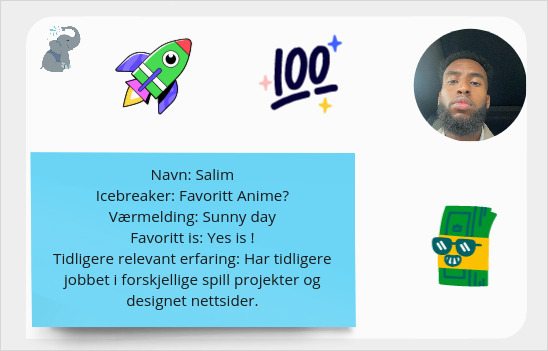
\includegraphics[scale=1]{icebreaker.png}
        \caption{A visual presentation of a team member}
        \label{fig:IB}
    \end{adjustwidth}
\end{figure}
\clearpage
\subsection{Expert interview and HMW\cite{WhatHowMight} questions}
The expert interviews allows us to learn about the background and context of a potential solution.
The goal of this exercise is to create \textbf{How Might We} questions.
The following is a selection of some of our most popular questions:
\begin{itemize}
    \item How might we present information in an effective and engaging way
    \item How might we make information easily editable
    \item How might we create a unique application
\end{itemize}
\subsection{Long term goals}
We were tasked with writing long term goals, on what the state of the application would be in two years.
The following are some of our most popular long term goals. 
\begin{itemize}
    \item In two years our application will be an important tool used by lots of buisnesses.
    \item In two years our application will be the standard for imformative displays
    \item In two years our application will be bug free
\end{itemize}
\subsection{Sprint questions}
Sprint questions are a set of assumptions about our application presented as questions.
The goal is to reflect on what we have to do to make this application a success.
The following are some of our most popular sprint questions:
\begin{itemize}
    \item Can we make an application that works with as many types of information displays as possible?
    \item Can we make an application where information can be modified quickly and easily?
    \item Can we make an application that is accessible for all?
\end{itemize}
\subsection{Map and area of focus}
We were tasked with finding out what problems are most pressing for achieving our goals.
This was done by creating a map of our \textbf{How Might We}\cite{WhatHowMight} questions.
\subsection{concept sketch}
Concept sketches were created based on the sprint questions from earlier tasks.
See \textit{Figure \ref{fig:SH}} for an example of one of the more popular concept sketches.
\begin{figure}[h]
    \begin{adjustwidth}{-1in}{-1in}
        \centering
        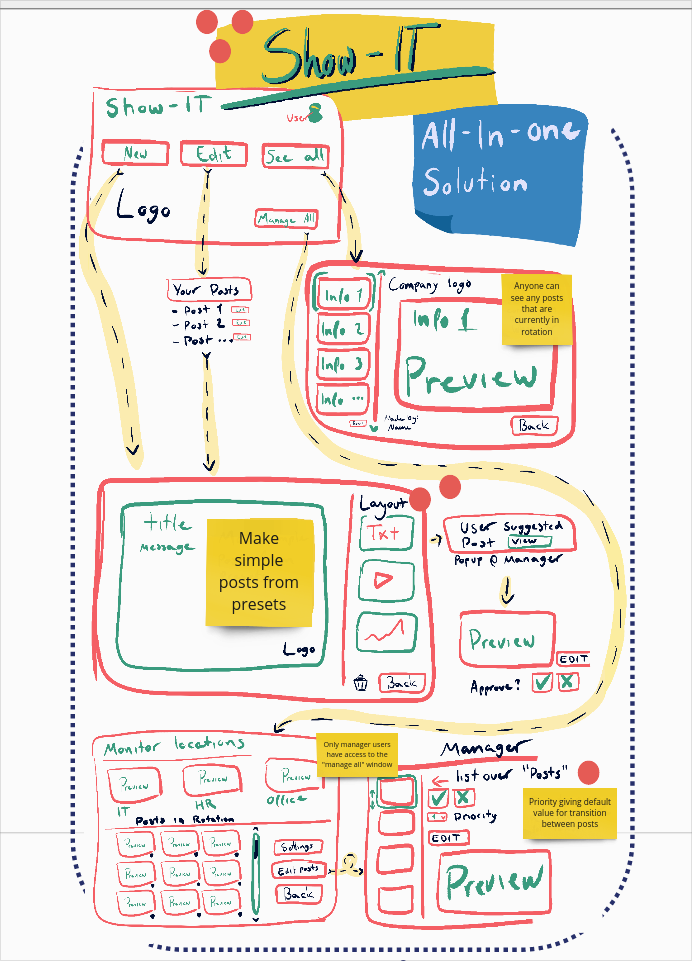
\includegraphics[scale=0.5]{show-it.png}
        \caption{An example of a concept sketch}
        \label{fig:SH}
    \end{adjustwidth}
\end{figure}
\clearpage
\subsection{lightning criticism}
lorem ipsum
\subsection{User test flow}
lorem ipsum
\subsubsection{Individual worksheets}
lorem ipsum
\subsubsection{Voting}
lorem ipsum
\subsection{Storyboard}
lorem ipsum

\section{Reflection}



\printbibliography
\end{document}